\section{Architectural Overview}\label{sec:arch}

The basic architecture to develop a system like this, regarding the existing TUMOnline system where you can check if a student is enrolled or not, will consist of the following parts:

\begin{itemize}
\item The Smartphone, including a NFC Chip as well as an internet connection to register with the service. The internet connection will be needed only one time to initialize the system
\item The Door system, also including a NFC Chip which can send and receive. A NFC Reader would not be enough due to simple replay attacks. The Door system also needs access to the internet or at least to an intranet to check if the student or the employee has access to the specific area and to get other informations for realizing security features like communication encryption. Therefore, some kind of computer is also needed, interacting with the NFC hardware as well as with the backend.
\item A backend system, which will take care of key generation and storage in case of a public-key system.

\item The TUMOnline system since is in the possession of the enrollment information of every student.
\end{itemize} 
 
 A complete overview of the basic architecture: \newline
 \begin{center}
 %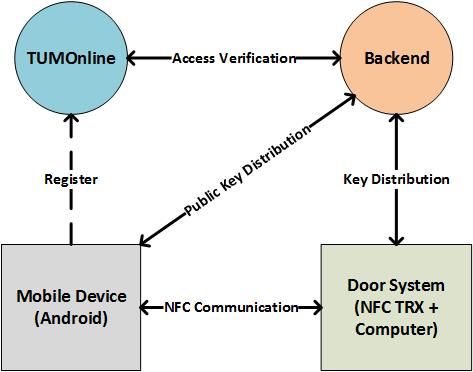
\includegraphics[scale=0.8]{basic_architecture.jpg}
\end{center}


\subsection{Registration with Backend}

\subsection{Authentication between Smartphone and NFC Transceiver}